% Options for packages loaded elsewhere
\PassOptionsToPackage{unicode}{hyperref}
\PassOptionsToPackage{hyphens}{url}
\PassOptionsToPackage{dvipsnames,svgnames,x11names}{xcolor}
%
\documentclass[
  letterpaper,
  DIV=11,
  numbers=noendperiod]{scrartcl}

\usepackage{amsmath,amssymb}
\usepackage{iftex}
\ifPDFTeX
  \usepackage[T1]{fontenc}
  \usepackage[utf8]{inputenc}
  \usepackage{textcomp} % provide euro and other symbols
\else % if luatex or xetex
  \usepackage{unicode-math}
  \defaultfontfeatures{Scale=MatchLowercase}
  \defaultfontfeatures[\rmfamily]{Ligatures=TeX,Scale=1}
\fi
\usepackage{lmodern}
\ifPDFTeX\else  
    % xetex/luatex font selection
\fi
% Use upquote if available, for straight quotes in verbatim environments
\IfFileExists{upquote.sty}{\usepackage{upquote}}{}
\IfFileExists{microtype.sty}{% use microtype if available
  \usepackage[]{microtype}
  \UseMicrotypeSet[protrusion]{basicmath} % disable protrusion for tt fonts
}{}
\makeatletter
\@ifundefined{KOMAClassName}{% if non-KOMA class
  \IfFileExists{parskip.sty}{%
    \usepackage{parskip}
  }{% else
    \setlength{\parindent}{0pt}
    \setlength{\parskip}{6pt plus 2pt minus 1pt}}
}{% if KOMA class
  \KOMAoptions{parskip=half}}
\makeatother
\usepackage{xcolor}
\setlength{\emergencystretch}{3em} % prevent overfull lines
\setcounter{secnumdepth}{-\maxdimen} % remove section numbering
% Make \paragraph and \subparagraph free-standing
\makeatletter
\ifx\paragraph\undefined\else
  \let\oldparagraph\paragraph
  \renewcommand{\paragraph}{
    \@ifstar
      \xxxParagraphStar
      \xxxParagraphNoStar
  }
  \newcommand{\xxxParagraphStar}[1]{\oldparagraph*{#1}\mbox{}}
  \newcommand{\xxxParagraphNoStar}[1]{\oldparagraph{#1}\mbox{}}
\fi
\ifx\subparagraph\undefined\else
  \let\oldsubparagraph\subparagraph
  \renewcommand{\subparagraph}{
    \@ifstar
      \xxxSubParagraphStar
      \xxxSubParagraphNoStar
  }
  \newcommand{\xxxSubParagraphStar}[1]{\oldsubparagraph*{#1}\mbox{}}
  \newcommand{\xxxSubParagraphNoStar}[1]{\oldsubparagraph{#1}\mbox{}}
\fi
\makeatother


\providecommand{\tightlist}{%
  \setlength{\itemsep}{0pt}\setlength{\parskip}{0pt}}\usepackage{longtable,booktabs,array}
\usepackage{calc} % for calculating minipage widths
% Correct order of tables after \paragraph or \subparagraph
\usepackage{etoolbox}
\makeatletter
\patchcmd\longtable{\par}{\if@noskipsec\mbox{}\fi\par}{}{}
\makeatother
% Allow footnotes in longtable head/foot
\IfFileExists{footnotehyper.sty}{\usepackage{footnotehyper}}{\usepackage{footnote}}
\makesavenoteenv{longtable}
\usepackage{graphicx}
\makeatletter
\newsavebox\pandoc@box
\newcommand*\pandocbounded[1]{% scales image to fit in text height/width
  \sbox\pandoc@box{#1}%
  \Gscale@div\@tempa{\textheight}{\dimexpr\ht\pandoc@box+\dp\pandoc@box\relax}%
  \Gscale@div\@tempb{\linewidth}{\wd\pandoc@box}%
  \ifdim\@tempb\p@<\@tempa\p@\let\@tempa\@tempb\fi% select the smaller of both
  \ifdim\@tempa\p@<\p@\scalebox{\@tempa}{\usebox\pandoc@box}%
  \else\usebox{\pandoc@box}%
  \fi%
}
% Set default figure placement to htbp
\def\fps@figure{htbp}
\makeatother

\usepackage{booktabs}
\usepackage{siunitx}
\KOMAoption{captions}{tableheading}
\makeatletter
\@ifpackageloaded{caption}{}{\usepackage{caption}}
\AtBeginDocument{%
\ifdefined\contentsname
  \renewcommand*\contentsname{Table of contents}
\else
  \newcommand\contentsname{Table of contents}
\fi
\ifdefined\listfigurename
  \renewcommand*\listfigurename{List of Figures}
\else
  \newcommand\listfigurename{List of Figures}
\fi
\ifdefined\listtablename
  \renewcommand*\listtablename{List of Tables}
\else
  \newcommand\listtablename{List of Tables}
\fi
\ifdefined\figurename
  \renewcommand*\figurename{Figure}
\else
  \newcommand\figurename{Figure}
\fi
\ifdefined\tablename
  \renewcommand*\tablename{Table}
\else
  \newcommand\tablename{Table}
\fi
}
\@ifpackageloaded{float}{}{\usepackage{float}}
\floatstyle{ruled}
\@ifundefined{c@chapter}{\newfloat{codelisting}{h}{lop}}{\newfloat{codelisting}{h}{lop}[chapter]}
\floatname{codelisting}{Listing}
\newcommand*\listoflistings{\listof{codelisting}{List of Listings}}
\makeatother
\makeatletter
\makeatother
\makeatletter
\@ifpackageloaded{caption}{}{\usepackage{caption}}
\@ifpackageloaded{subcaption}{}{\usepackage{subcaption}}
\makeatother

\usepackage{bookmark}

\IfFileExists{xurl.sty}{\usepackage{xurl}}{} % add URL line breaks if available
\urlstyle{same} % disable monospaced font for URLs
\hypersetup{
  pdftitle={Analysis of International Debt Statistics},
  colorlinks=true,
  linkcolor={blue},
  filecolor={Maroon},
  citecolor={Blue},
  urlcolor={Blue},
  pdfcreator={LaTeX via pandoc}}


\title{Analysis of International Debt Statistics}
\author{}
\date{}

\begin{document}
\maketitle


\subsection{Executive Summary}\label{executive-summary}

This note analyses sovereign debt vulnerability across developing
countries using cross-sectional data from the World Bank's International
Debt Statistics (IDS) for 2023. The analysis finds that \textbf{a
substantial share of developing countries --- particularly in
Sub-Saharan Africa and Latin America --- exceed key IMF/World Bank
stress thresholds} for external debt. Higher debt burdens, costlier
borrowing terms, and elevated short-term debt shares are the primary
drivers of debt service pressure. The shift away from concessional
multilateral financing toward market-rate instruments is compressing the
financial space available to governments and increasing rollover risk.
Urgent reforms to the sovereign debt architecture are needed to restore
sustainable financing pathways for the most vulnerable countries.

\begin{center}\rule{0.5\linewidth}{0.5pt}\end{center}

\subsection{1. Background and
Motivation}\label{background-and-motivation}

The global sovereign debt landscape has deteriorated markedly since the
COVID-19 pandemic. Rising interest rates in advanced economies, currency
depreciations, and slowing growth have compressed fiscal space across
the developing world. The number of low- and middle-income countries at
high risk of --- or already in --- debt distress has risen to
historically elevated levels, yet the international debt restructuring
architecture remains fragmented and slow.

This analysis uses the World Bank's \textbf{International Debt
Statistics (IDS)} database --- the most comprehensive publicly available
dataset on external debt stocks, flows, and creditor composition for
developing countries --- to provide a systematic cross-sectional
snapshot of debt vulnerability in 2023. The goal is to identify
countries and patterns of concern and to draw policy-relevant
conclusions about the evolving structure of developing country debt.

\begin{center}\rule{0.5\linewidth}{0.5pt}\end{center}

\subsection{2. Data and Methodology}\label{data-and-methodology}

\subsubsection{2.1 Data Source}\label{data-source}

All data are drawn from the \textbf{World Bank International Debt
Statistics (IDS), 2023}. The IDS covers external debt stocks and flows
for low- and middle-income countries, disaggregated by creditor type
(multilateral, bilateral, bonds, commercial banks) and debt category
(public and publicly guaranteed, private non-guaranteed, short-term).

The following indicators were used:

\begin{longtable}[]{@{}
  >{\raggedright\arraybackslash}p{(\linewidth - 4\tabcolsep) * \real{0.3611}}
  >{\raggedright\arraybackslash}p{(\linewidth - 4\tabcolsep) * \real{0.2500}}
  >{\raggedright\arraybackslash}p{(\linewidth - 4\tabcolsep) * \real{0.3889}}@{}}
\toprule\noalign{}
\begin{minipage}[b]{\linewidth}\raggedright
Indicator
\end{minipage} & \begin{minipage}[b]{\linewidth}\raggedright
Code
\end{minipage} & \begin{minipage}[b]{\linewidth}\raggedright
Description
\end{minipage} \\
\midrule\noalign{}
\endhead
\bottomrule\noalign{}
\endlastfoot
External debt (\% GNI) & DT.DOD.DECT.GN.ZS & Primary sustainability
ratio \\
Total debt service (\% exports) & DT.TDS.DECT.EX.ZS & Debt repayment
burden \\
Short-term debt share & DT.DOD.DSTC.ZS & Rollover and liquidity risk \\
Reserves (months of imports) & FI.RES.TOTL.MO & External buffer
adequacy \\
Multilateral debt & DT.DOD.MLAT.CD & MDB financing \\
Bilateral debt & DT.DOD.BLAT.CD & Government-to-government lending \\
Bond debt & DT.DOD.PBND.CD & Market financing \\
Commercial bank debt & DT.DOD.PCBK.CD & Private creditor exposure \\
Concessional debt share & DT.DOD.ALLC.CD & Concessionality of
portfolio \\
Grant element on new loans & DT.GRE.DPPG & Terms on new commitments \\
Average interest rate & DT.INR.DPPG & Cost of new borrowing \\
\end{longtable}

\emph{Source: World Bank IDS Databank, 2025 edition.}

\subsubsection{2.2 Country Coverage}\label{country-coverage}

The sample covers all low-income, lower-middle-income, and
upper-middle-income countries for which data are available in 2023.
Aggregate and regional groupings provided by the World Bank are excluded
to ensure country-level analysis.

\subsubsection{2.3 Risk Classification}\label{risk-classification}

Countries are classified into three risk tiers based on IMF and World
Bank debt sustainability thresholds:

\begin{itemize}
\tightlist
\item
  \textbf{High Risk}: External debt \textgreater{} 60\% of GNI
  \textbf{and} debt service \textgreater{} 20\% of exports
\item
  \textbf{Elevated Risk}: External debt \textgreater{} 40\% of GNI
  \textbf{or} debt service \textgreater{} 15\% of exports
\item
  \textbf{Moderate}: Below both thresholds
\end{itemize}

\subsubsection{2.4 Regression Model}\label{regression-model}

To identify the key drivers of debt service burden, an OLS regression
was estimated with total debt service (\% of exports) as the dependent
variable:

\(\text{Debt Service}_i = \beta_0 + \beta_1\,\text{Debt/GNI}_i + \beta_2\,\text{Short-term share}_i + \beta_3\,\text{Reserves}_i + \beta_4\,\text{Concessional share}_i + \beta_5\,\text{Grant element}_i + \varepsilon_i\)

\begin{center}\rule{0.5\linewidth}{0.5pt}\end{center}

\subsection{3. Results}\label{results}

\subsubsection{3.1 Debt Vulnerability: A Cross-Country
View}\label{debt-vulnerability-a-cross-country-view}

\begin{figure}[H]

{\centering 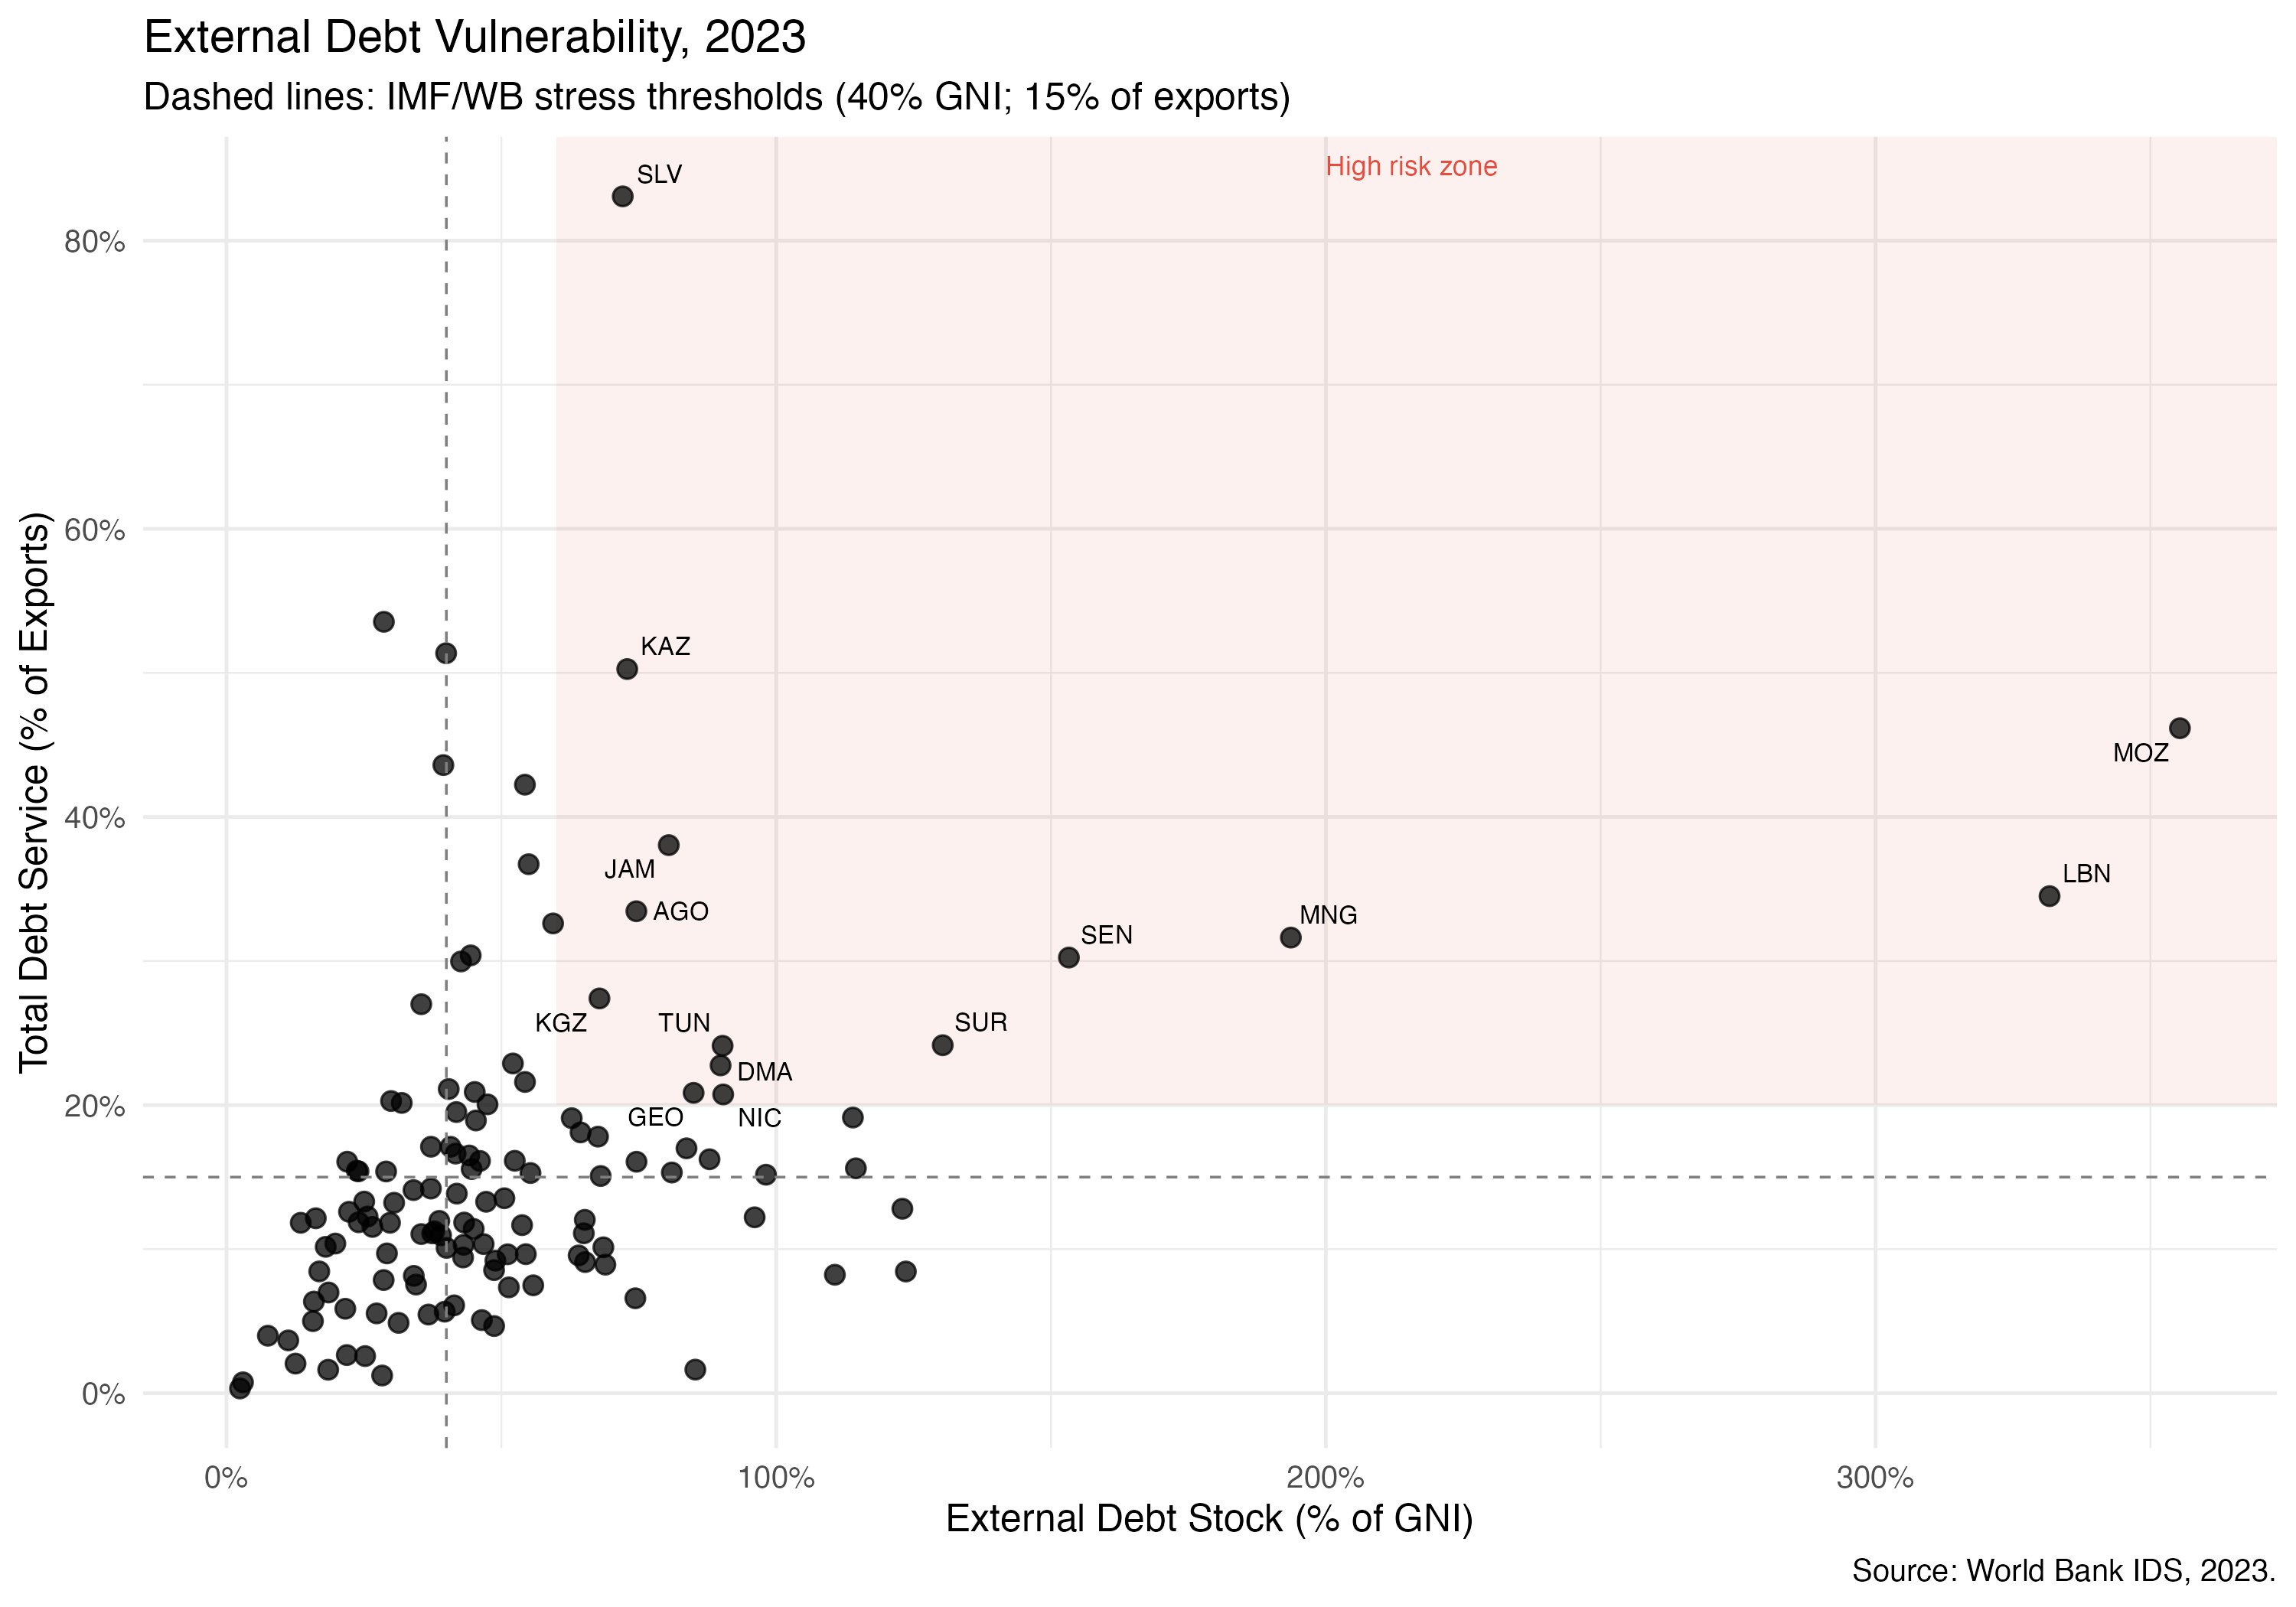
\includegraphics[width=1\linewidth,height=\textheight,keepaspectratio]{p1_vulnerability.png}

}

\caption{Figure 1. External Debt Vulnerability, 2023}

\end{figure}%

Note: Dashed lines indicate IMF/World Bank stress thresholds: 40\% GNI
(vertical) and 15\% of exports (horizontal). Red shading marks the
high-risk zone. Country codes label countries classified as High Risk.
Source: World Bank IDS, 2023.

Figure 1 plots each country's external debt stock (as a share of GNI)
against its total debt service ratio (as a share of exports). Several
features stand out:

\begin{itemize}
\tightlist
\item
  \textbf{Lebanon (LBN) and Mozambique (MOZ)} are extreme outliers, with
  external debt stocks exceeding 300\% of GNI and debt service ratios
  above 30--45\% of exports --- far beyond any conventional
  sustainability benchmark.
\item
  \textbf{El Salvador (SLV)} stands out for its acute debt service
  burden (over 80\% of exports) despite a moderate debt stock,
  reflecting the compressed maturity structure and high interest costs
  of its dollarised economy.
\item
  \textbf{Mongolia (MNG), Senegal (SEN), and Suriname (SUR)} all sit in
  or near the high-risk quadrant, consistent with their ongoing
  engagement with IMF programmes and debt restructuring processes.
\item
  The majority of countries cluster at debt levels below 60\% of GNI,
  but many already exceed the 15\% debt service threshold --- indicating
  that service pressure is widespread even at seemingly moderate stock
  levels.
\end{itemize}

\textbf{Finding 1:} Debt service pressure is more widespread than debt
stock ratios alone suggest. A significant share of developing countries
exceed the 15\% export threshold for debt service even when their
aggregate debt stocks appear manageable, pointing to unfavourable loan
terms and compressed maturities as key drivers.

\begin{center}\rule{0.5\linewidth}{0.5pt}\end{center}

\subsubsection{3.2 Creditor Composition: The Structural Shift Away from
Multilaterals}\label{creditor-composition-the-structural-shift-away-from-multilaterals}

\begin{figure}[H]

{\centering 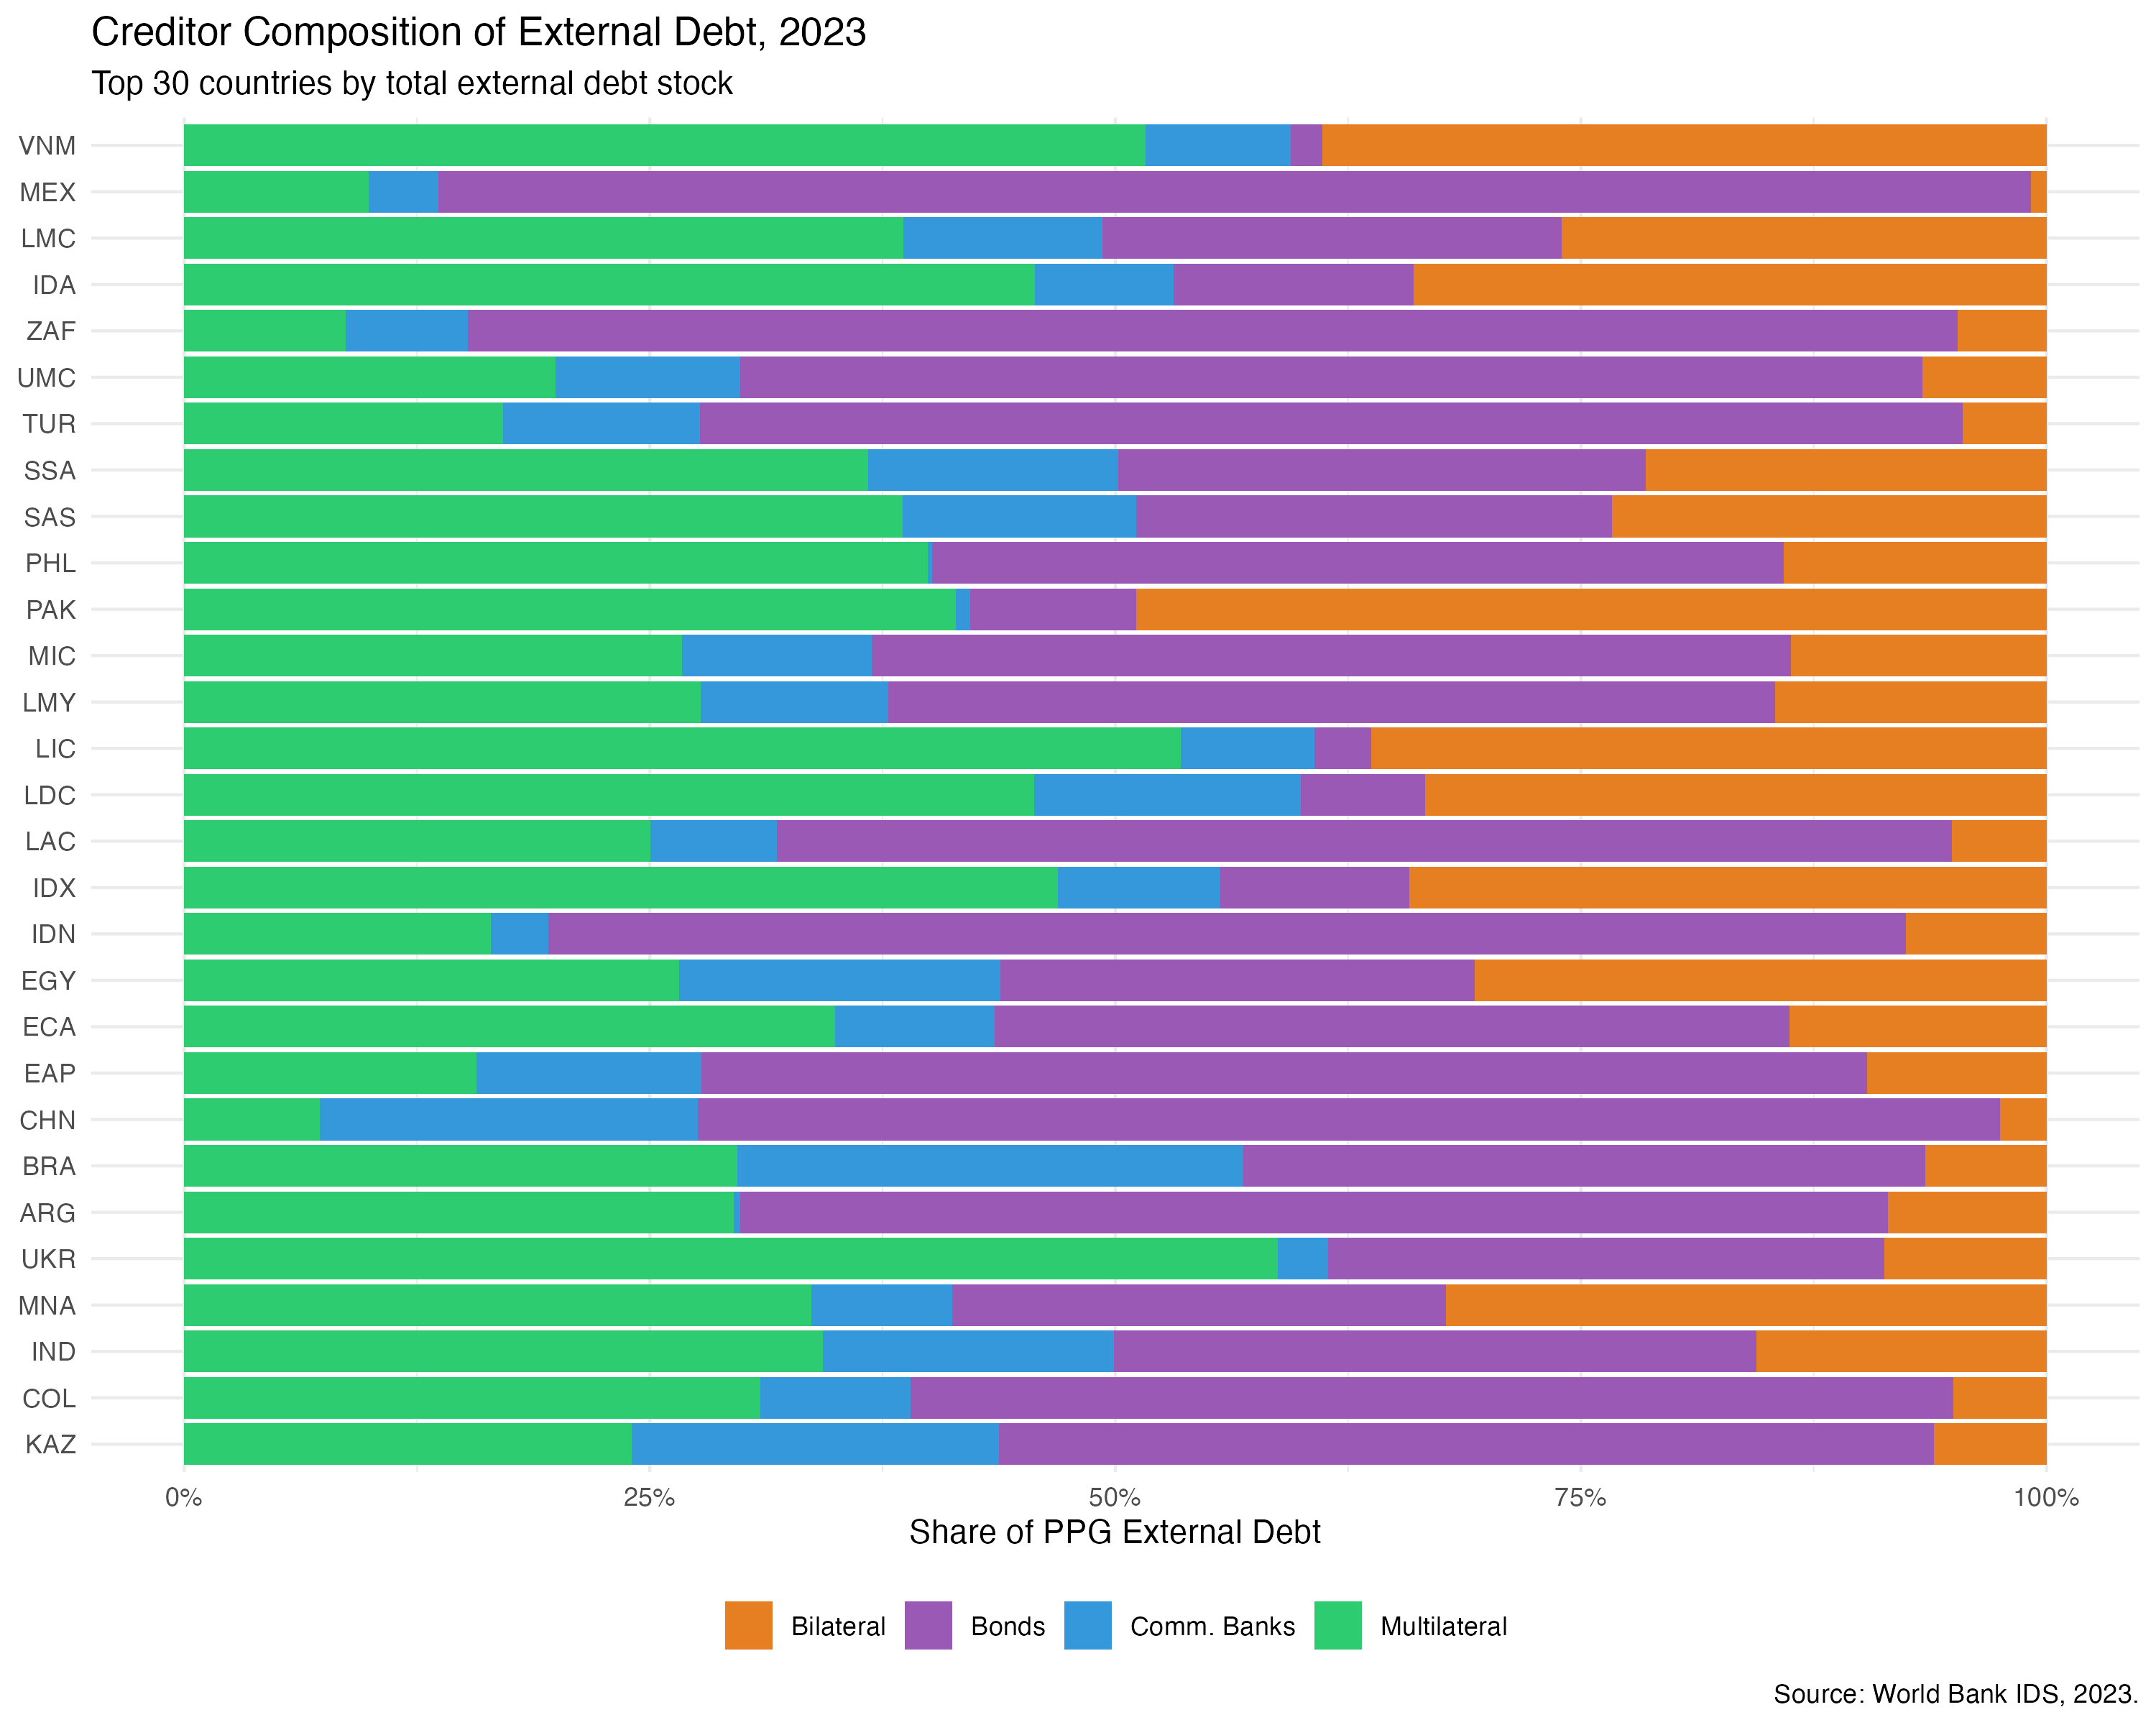
\includegraphics[width=1\linewidth,height=\textheight,keepaspectratio]{p2_creditors.png}

}

\caption{Figure 2. Creditor Composition of External Debt, Top 30
Countries, 2023}

\end{figure}%

Note: Shows the 30 countries with the largest total external debt
stocks. Shares are of public and publicly guaranteed (PPG) external
debt. Source: World Bank IDS, 2023.

Figure 2 reveals striking heterogeneity in creditor composition across
developing countries:

\begin{itemize}
\tightlist
\item
  \textbf{Bond financing dominates} among upper-middle-income and larger
  lower-middle-income economies (Argentina, Brazil, Colombia, Mexico,
  Turkey), where private market access exists but comes at market rates
  with shorter maturities.
\item
  \textbf{Multilateral creditors} remain the primary source for many
  lower-income countries --- particularly in South Asia and Sub-Saharan
  Africa --- reflecting continued IDA and MDB engagement.
\item
  \textbf{Bilateral creditors} (including China) hold a large share of
  debt in several Sub-Saharan African countries and in Vietnam,
  consistent with Belt and Road Initiative (BRI) financing patterns
  documented elsewhere.
\item
  The presence of \textbf{commercial banks} is most pronounced in East
  Asia and Latin America, adding an additional layer of private creditor
  coordination complexity in any future restructuring.
\end{itemize}

\textbf{Finding 2:} The creditor landscape is highly fragmented.
Countries with large bilateral and bond exposures face coordination
challenges in any restructuring scenario, as these creditors operate
under different legal frameworks and have historically resisted
comparable treatment --- a core challenge identified in the G20 Common
Framework.

\begin{center}\rule{0.5\linewidth}{0.5pt}\end{center}

\subsubsection{3.3 Liquidity Risk: Reserves vs Short-Term
Debt}\label{liquidity-risk-reserves-vs-short-term-debt}

\begin{figure}[H]

{\centering 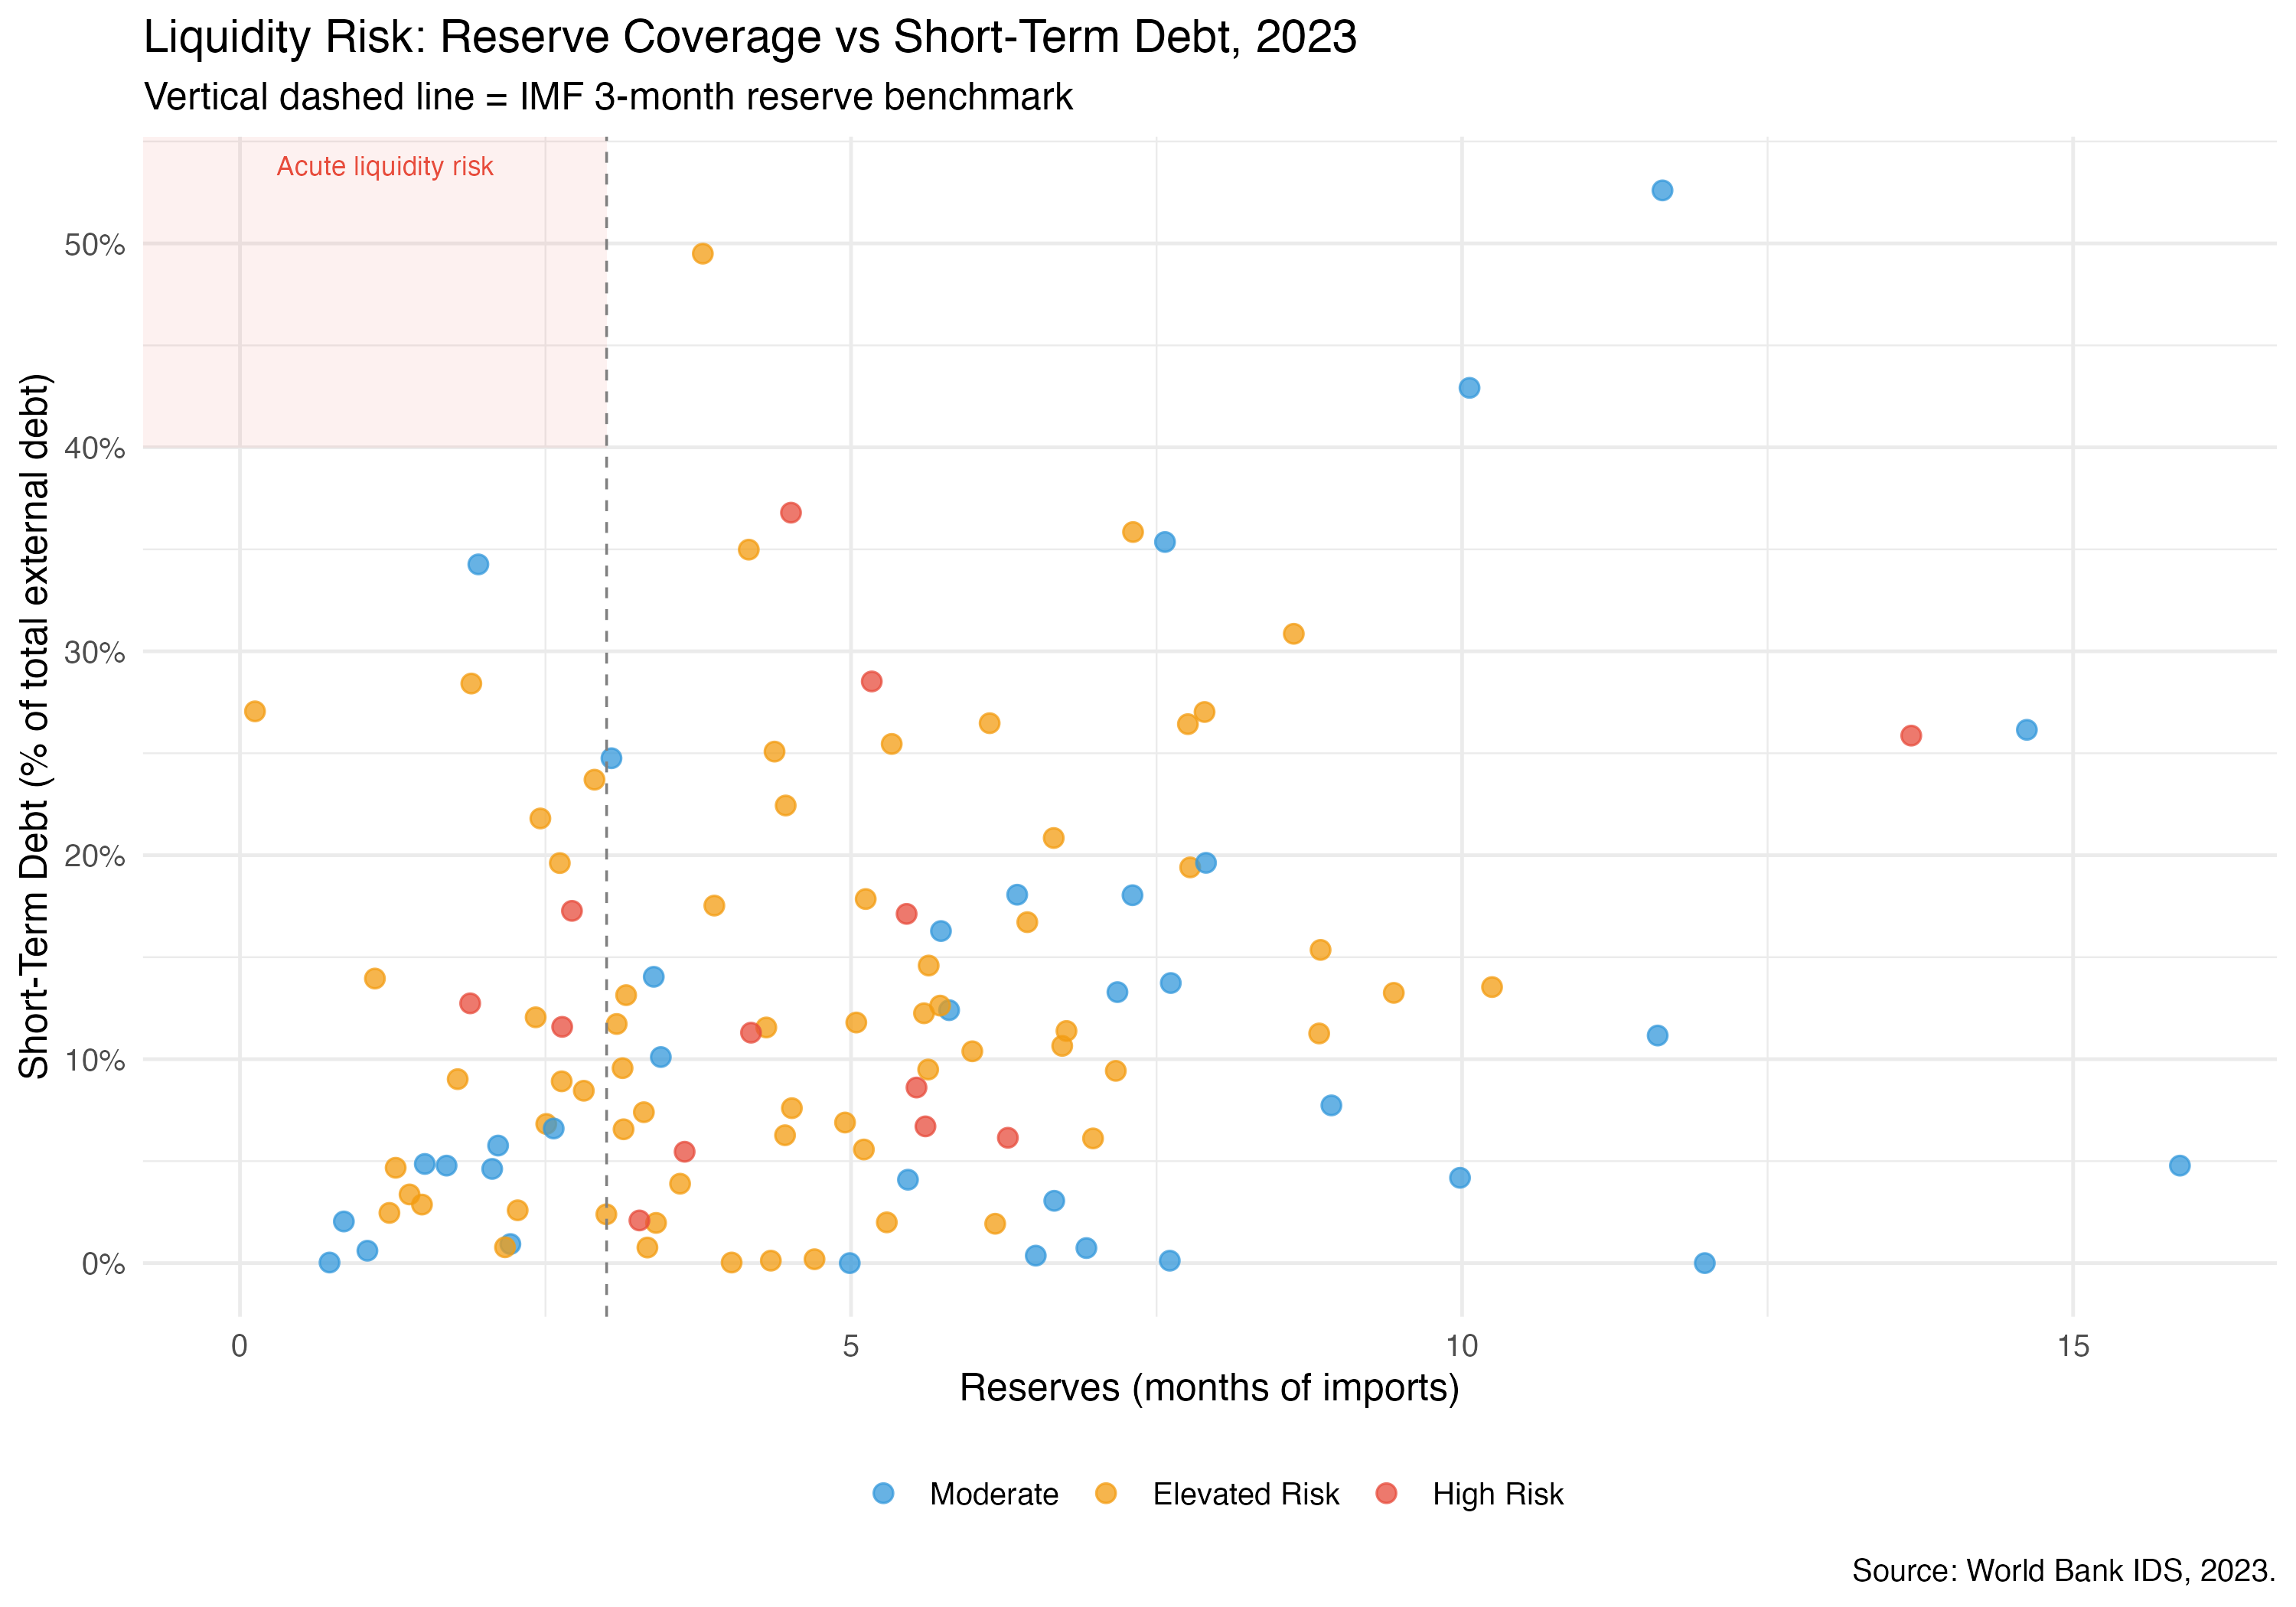
\includegraphics[width=1\linewidth,height=\textheight,keepaspectratio]{p3_liquidity.png}

}

\caption{Figure 3. Liquidity Risk: Reserve Coverage vs Short-Term Debt,
2023}

\end{figure}%

Note: The vertical dashed line marks the IMF's 3-month reserve adequacy
benchmark. The red-shaded region indicates acute liquidity risk (low
reserves combined with high short-term debt). Source: World Bank IDS,
2023.

Figure 3 plots reserve coverage against the share of external debt that
is short-term, providing a liquidity risk lens distinct from the
solvency analysis in Figure 1:

\begin{itemize}
\tightlist
\item
  Several countries hold \textbf{fewer than 3 months of import cover}
  (below the IMF benchmark), making them acutely vulnerable to external
  shocks or sudden capital flow reversals.
\item
  Countries with \textbf{high short-term debt shares} (above 40\%) face
  significant rollover risk --- even if their total debt stock appears
  manageable, a loss of market access could trigger immediate liquidity
  distress.
\item
  Interestingly, several \textbf{Moderate-risk countries} (blue) have
  very low short-term debt shares, reflecting the concessional nature of
  their borrowing (long-maturity IDA and bilateral loans), while
  \textbf{Elevated-risk countries} cluster at higher short-term shares.
\end{itemize}

\textbf{Finding 3:} Reserve inadequacy and high short-term debt shares
are concentrated among Elevated Risk countries, creating a dangerous
combination where any deterioration in market sentiment could rapidly
convert a liquidity event into a solvency crisis.

\begin{center}\rule{0.5\linewidth}{0.5pt}\end{center}

\subsubsection{3.4 Borrowing Terms: The Retreat of Concessional
Finance}\label{borrowing-terms-the-retreat-of-concessional-finance}

\begin{figure}[H]

{\centering 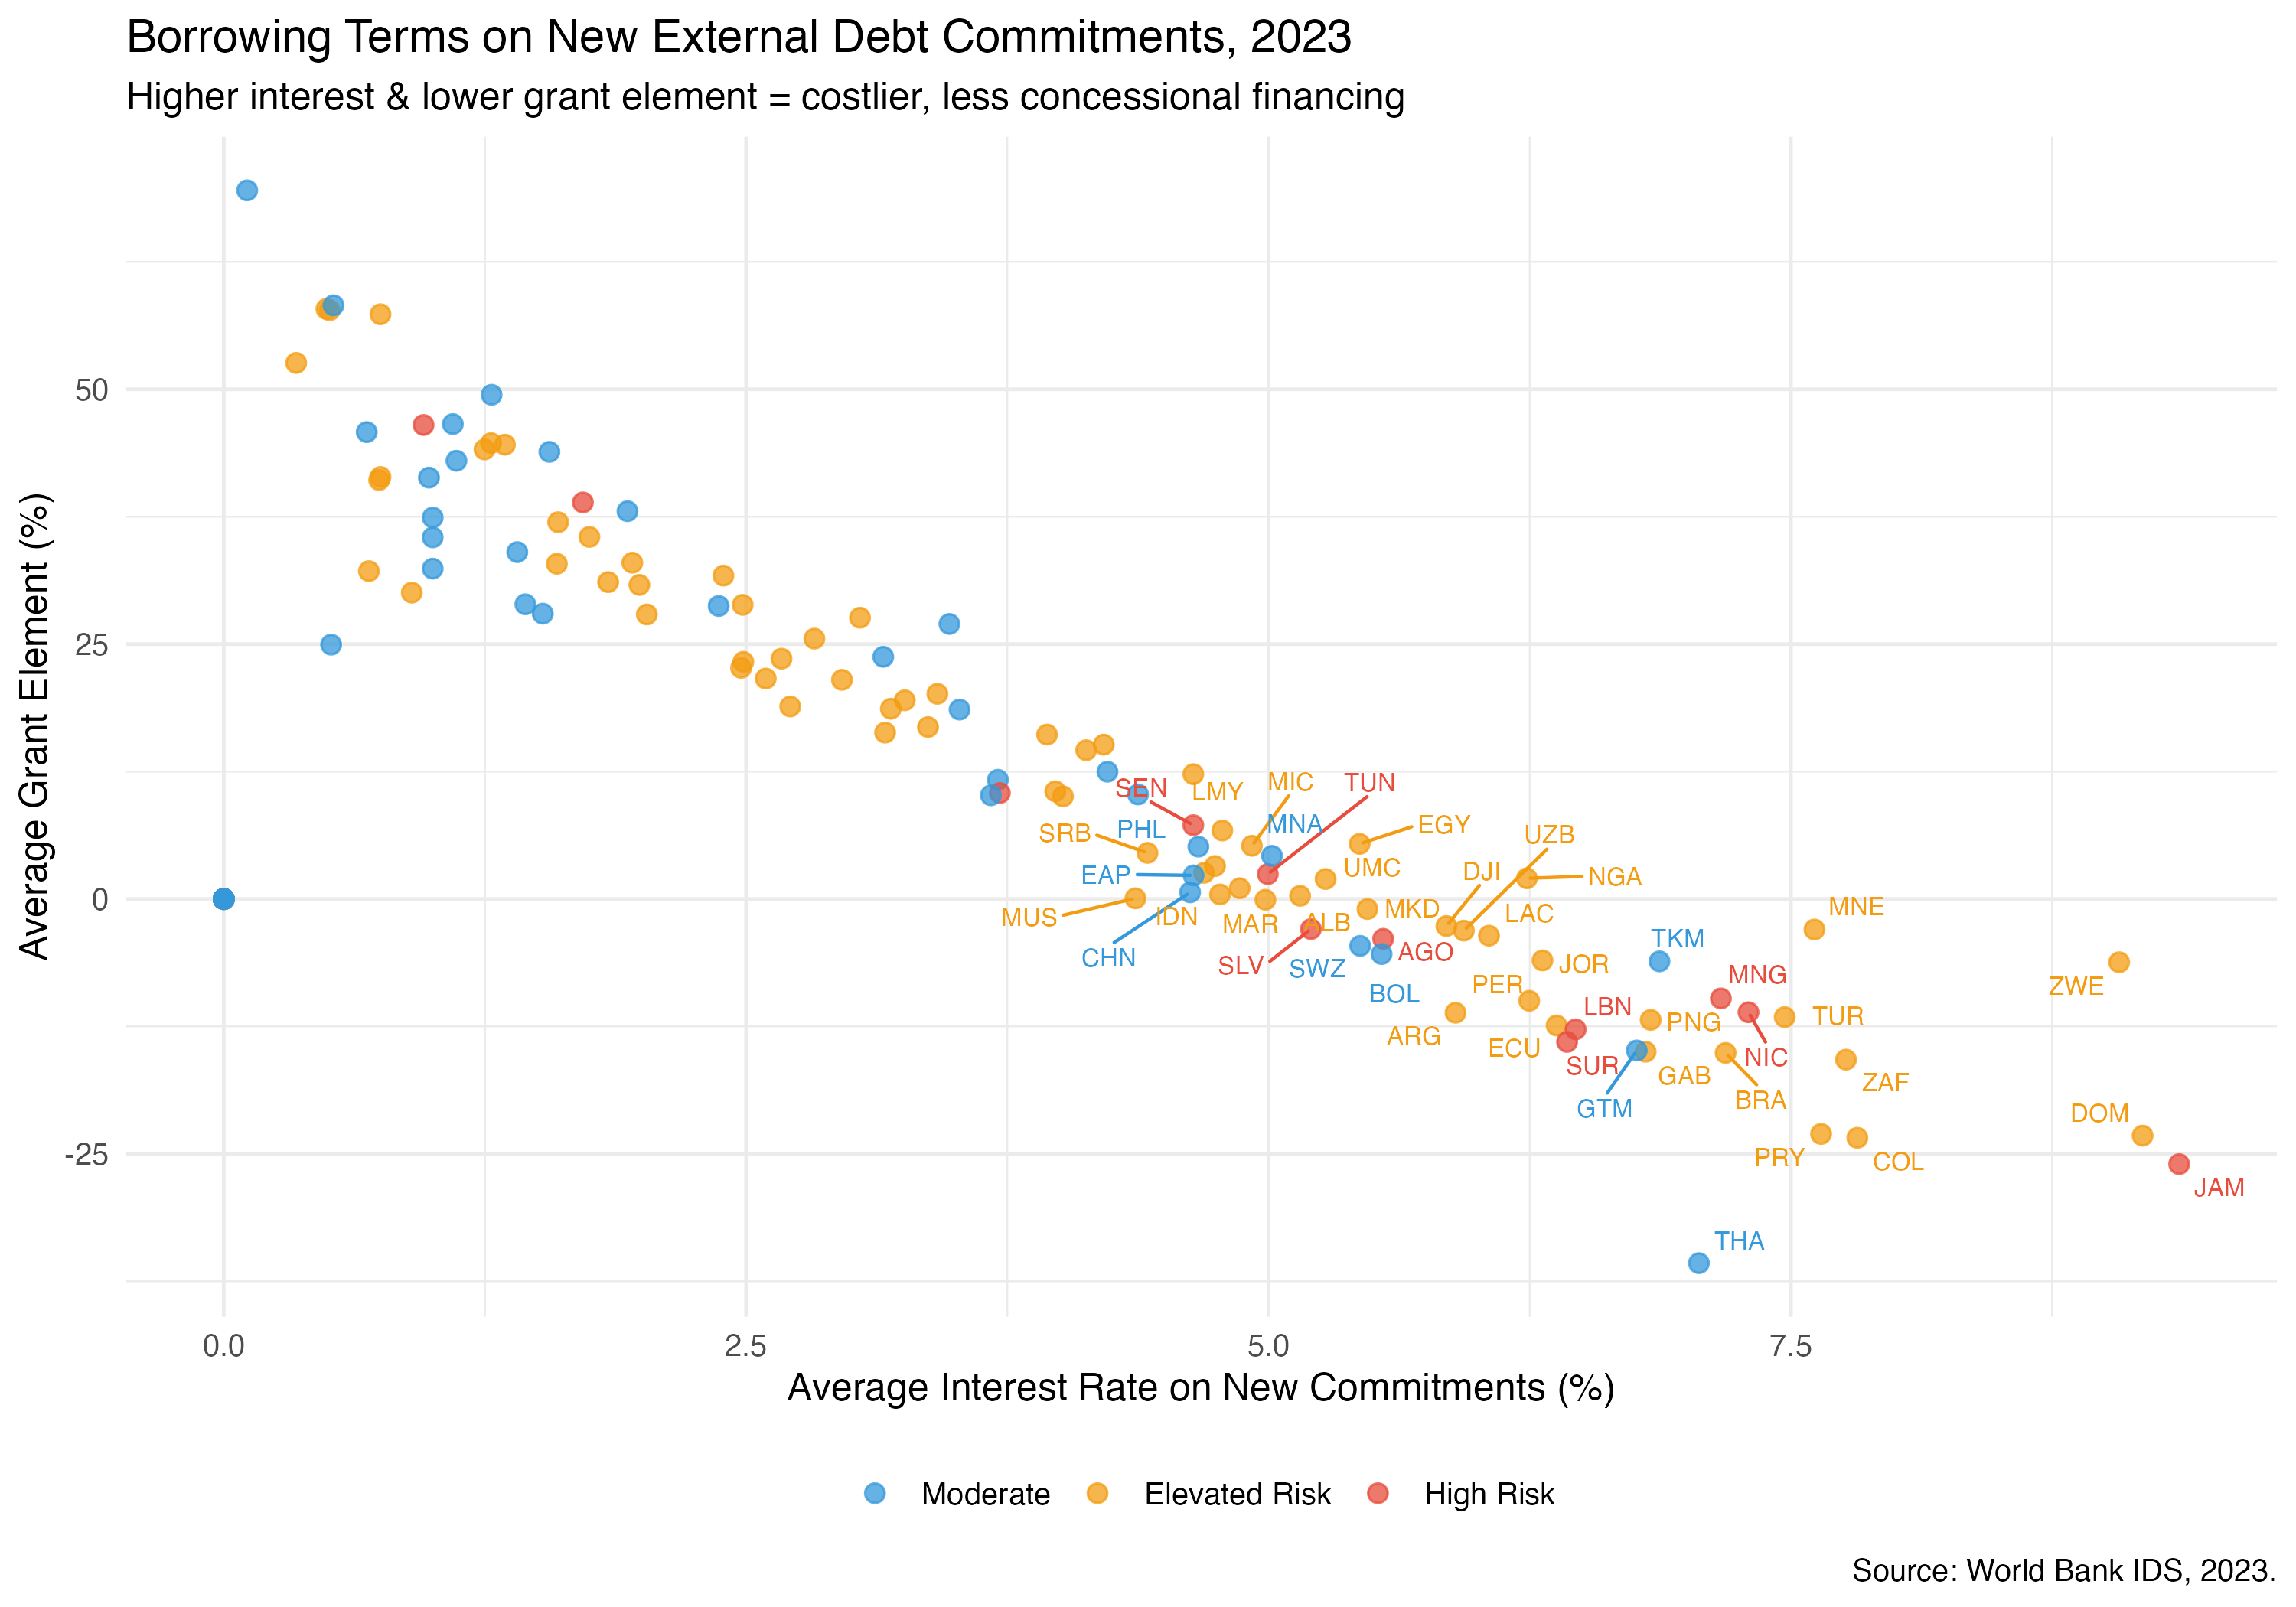
\includegraphics[width=1\linewidth,height=\textheight,keepaspectratio]{p4_loan_terms.png}

}

\caption{Figure 4. Borrowing Terms on New External Debt Commitments,
2023}

\end{figure}%

Note: The grant element measures the concessionality of a loan relative
to a market reference rate. Negative values indicate loans with
above-market interest rates. Labelled countries have particularly high
interest rates or very low grant elements. Source: World Bank IDS, 2023.

Figure 4 examines the terms on \textbf{new} external debt commitments
--- a forward-looking indicator of the trajectory of debt
sustainability:

\begin{itemize}
\tightlist
\item
  There is a \textbf{strong negative relationship} between average
  interest rates and grant elements, as expected: higher interest loans
  carry lower concessionality.
\item
  Several countries --- including \textbf{Jamaica (JAM), Zimbabwe (ZWE),
  Montenegro (MNE), and Dominican Republic (DOM)} --- are committing to
  new debt at interest rates above 7.5\% with negative grant elements,
  meaning they are borrowing on terms \textbf{worse than the market
  reference rate}.
\item
  Countries in the \textbf{Moderate risk} category (blue) tend to
  cluster at low interest rates and high grant elements, reflecting
  continued access to IDA and other concessional windows.
\item
  The \textbf{High Risk} group is scattered across the interest rate
  spectrum, suggesting that even distressed countries retain some access
  to new borrowing --- often at punishing terms.
\end{itemize}

\textbf{Finding 4:} The retreat of concessional finance is pushing many
developing countries into market-rate borrowing at precisely the moment
when their debt positions are most fragile. Countries committing to new
debt with negative grant elements are locking in a structural
deterioration of their debt dynamics.

\begin{center}\rule{0.5\linewidth}{0.5pt}\end{center}

\subsection{4. Regression Analysis: Drivers of Debt Service
Burden}\label{regression-analysis-drivers-of-debt-service-burden}

To disentangle the determinants of debt service pressure, an OLS
regression was estimated on the cross-section of developing countries
with complete data (n = 111).

\subsubsection{4.1 Results}\label{results-1}

\begin{table}[!htbp] \centering 
  \caption{} 
  \label{} 
\begin{tabular}{@{\extracolsep{5pt}}lc} 
\\[-1.8ex]\hline 
\hline \\[-1.8ex] 
 & \multicolumn{1}{c}{\textit{Dependent variable:}} \\ 
\\[-1.8ex] & Debt Service Burden \\ 
\hline \\[-1.8ex] 
 External debt (\% GNI) & 0.084$^{***}$ \\ 
  & (0.022) \\ 
  & \\ 
 Short-term debtshare & $-$0.059 \\ 
  & (0.107) \\ 
  & \\ 
 Reserves(monthsimports) & $-$0.613 \\ 
  & (0.389) \\ 
  & \\ 
 Concessional share & $-$10.209 \\ 
  & (8.086) \\ 
  & \\ 
 Grant element & $-$0.193$^{***}$ \\ 
  & (0.065) \\ 
  & \\ 
 Constant & 19.667$^{***}$ \\ 
  & (3.119) \\ 
  & \\ 
\hline \\[-1.8ex] 
Observations & 111 \\ 
R$^{2}$ & 0.278 \\ 
Adjusted R$^{2}$ & 0.244 \\ 
\hline 
\hline \\[-1.8ex] 
\textit{Note:}  & \multicolumn{1}{r}{$^{*}$p$<$0.1; $^{**}$p$<$0.05; $^{***}$p$<$0.01} \\ 
\end{tabular} 
\end{table}

\subsubsection{4.2 Interpretation}\label{interpretation}

Two variables are statistically significant predictors of debt service
burden:

\textbf{External debt stock (\% GNI)} is the strongest and most
precisely estimated predictor. A 10 percentage point increase in the
debt-to-GNI ratio is associated with an additional \textbf{0.84
percentage points} of debt service as a share of exports, holding other
factors constant. This confirms that stock accumulation directly
translates into service pressure.

\textbf{Grant element on new commitments} is the second significant
predictor, with a negative sign: a 10 percentage point increase in the
grant element on new loans is associated with a \textbf{1.93 percentage
point reduction} in debt service burden. This finding is particularly
policy-relevant --- it quantifies the direct benefit of concessional
financing for near-term debt sustainability, and underscores the cost of
the structural shift toward market-rate borrowing documented in Figure
4.

The \textbf{reserve coverage, short-term debt share, and concessional
stock share} are in the expected direction but do not reach conventional
significance thresholds, likely due to cross-country heterogeneity and
the relatively small sample. The concessional share result (-10.2, p =
0.21) is economically substantial and warrants further investigation
with a larger or panel dataset.

The model explains \textbf{27.8\% of the cross-country variation} in
debt service ratios --- a reasonable fit for a parsimonious
cross-sectional specification, and consistent with the expectation that
country-specific factors not captured here (exchange rate dynamics,
domestic fiscal conditions, debt maturity profiles) also play important
roles.

\textbf{Finding 5:} The regression confirms two robust,
policy-actionable drivers of debt service burden: (1) the level of debt
accumulation, and (2) the terms on which new borrowing is contracted.
Countries that maintain access to concessional finance face materially
lower service burdens, all else equal --- a direct argument for
expanding MDB lending capacity and preserving grant windows.

\begin{center}\rule{0.5\linewidth}{0.5pt}\end{center}

\subsection{5. Policy Implications}\label{policy-implications}

\textbf{1. Strengthen the G20 Common Framework for debt restructuring.}
The concentration of bilateral and bond creditors identified in Figure 2
--- with heterogeneous legal frameworks and incentive structures ---
explains the slow pace of restructuring under the Common Framework.
Credible burden-sharing rules and tighter timelines for comparability of
treatment are essential.

\textbf{2. Expand concessional lending capacity at multilateral
development banks.} The regression results directly quantify the fiscal
benefit of concessional financing. The ongoing capital adequacy reviews
at the World Bank and regional MDBs should prioritise expanding IDA and
concessional windows, particularly for countries being priced out of
sovereign bond markets.

\textbf{3. Implement early warning systems based on composite
indicators.} This analysis demonstrates that debt stock ratios alone are
insufficient --- countries can face acute service pressure at moderate
debt levels if terms are unfavourable or maturities compressed. A
composite early warning framework incorporating debt service ratios,
reserve adequacy, short-term share, and grant element trends would
improve detection of countries approaching distress.

\textbf{4. Address the negative grant element problem urgently.} Several
countries identified in Figure 4 are accessing new financing at
below-zero grant elements --- effectively borrowing on terms worse than
market. This is inconsistent with debt sustainability and likely
reflects constrained alternatives. Expanding emergency concessional
facilities (including IMF RST and MDB crisis windows) would reduce this
distortion.

\begin{center}\rule{0.5\linewidth}{0.5pt}\end{center}

\subsection{6. Limitations and
Extensions}\label{limitations-and-extensions}

This analysis is cross-sectional and uses a single year (2023), which
limits causal inference and the ability to track trajectories. Key
extensions would include:

\begin{itemize}
\tightlist
\item
  \textbf{Panel estimation} using IDS data from 2000--2023 to exploit
  within-country variation and control for unobserved heterogeneity
\item
  \textbf{Creditor-specific analysis} --- particularly separating
  Chinese bilateral lending from Paris Club bilateral creditors, which
  have very different restructuring dynamics
\item
  \textbf{Domestic debt} --- the IDS covers only external debt; domestic
  debt obligations are not captured but are increasingly relevant for
  frontier market economies
\item
  \textbf{Integration with IMF DSA outputs} --- combining IDS data with
  IMF Debt Sustainability Analysis classifications would allow
  validation of the risk flags used here
\end{itemize}

\begin{center}\rule{0.5\linewidth}{0.5pt}\end{center}

\subsection{7. Data and Replication}\label{data-and-replication}

All data are publicly available from the
\href{https://databank.worldbank.org/source/international-debt-statistics}{World
Bank IDS Databank}. Analysis was conducted in R using the
\texttt{tidyverse}, \texttt{ggplot2}, \texttt{scales}, \texttt{ggrepel},
and \texttt{countrycode} packages. The full replication code is
available on request.

\begin{center}\rule{0.5\linewidth}{0.5pt}\end{center}




\end{document}
